\section{Arquitectura del sistema}

En la Figura \ref{arq} se muestra una visión de la arquitectura del sistema. Se
trata de una arquitectura cliente-servidor a través de servicios web. Su implementación se ha llevado a cabo usando el framework Google Web Toolkit(GWT).
El servidor proporciona e implementa una serie de operaciones a través de un interfaz que extiende de ``Remote Service''. Este servidor web es un mero proxy para los clientes web, ya que no contiene la funcionalidad del servidor como tal, que la sigue mantiendo el servidor de escritorio.

 \begin{figure}[h]
 \centering
 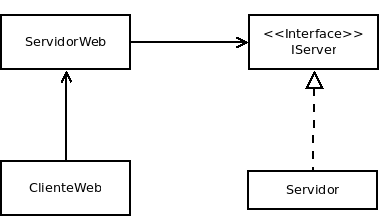
\includegraphics[scale=0.65]{img/arq.png}
 \caption{Interacción entre cliente web, servidor web y servidor de escritorio}
 \label{arq}
 \end{figure}

Los clientes solicitan los servicios que el servidor web ofrece usando la interfaz proporcionada y este, se comunica a través de RMI con el servidor de escritorio. En esta comuncación el servidor web actúa en rol de cliente del servidor de escritorio, que es el componente que contiene toda la lógica propia del servidor como tal. Esta comunicación se realiza mediante RMI.
Por lo tanto los flujos de información que se producen, se resumen en:
\begin{itemize}
 \item Clientes web a servidor web.
\item Servidor web con rol de cliente de escritorio a servidor de escritorio.
\end{itemize}
En la Figura \ref{arq} se puede observar la arquitectura descrita.
Al igual que en la anterior práctica, la lógica del juego reside en la parte del cliente web.

En la siguiente figura, se puede apreciar la arquitectura de la aplicación web, conformada tanto por el servidor web y el cliente web.

 \begin{figure}[h]
 \centering
 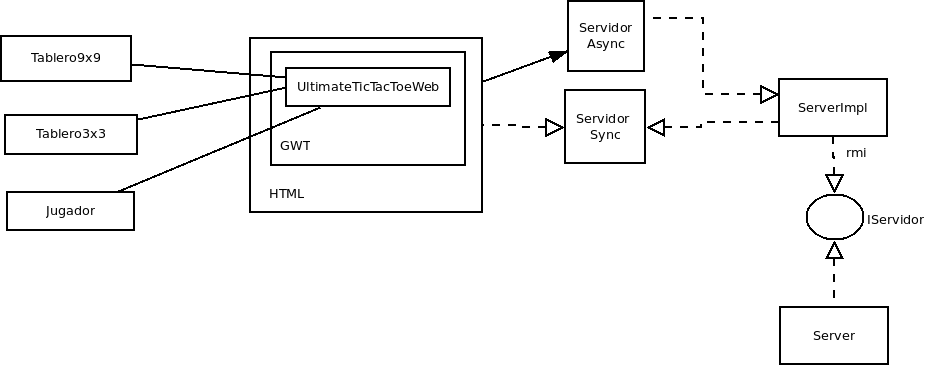
\includegraphics[scale=0.55]{img/diagrama.png}
 \caption{Arquitectura del sistema}
 \label{arq_sistema}
 \end{figure}

\subsection{Arquitectura del Servidor web}

Como se puede apreciar en la Figura \ref{arq_sistema}, el servidor web está basado únicamente en una capa de comunicación ya que no posee dominio o persistencia alguna.

\begin{itemize}
  \item \emph{Comunicación:} La clase encargada de esta función es \emph{ServerImpl}. Implementa la interfaz del Servidor Síncrono en la parte web y usa la interfaz del Servidor RMI, permitiendo la comunicación con otros clientes, tanto web como de escritorio.
\end{itemize}

\subsection{Arquitectura del Cliente web}

En la Figura \ref{arq_sistema} se muestra la arquitectura multicapa del servidor:

\begin{itemize}
 \item \emph{Comunicación:} La clase encargada de estas tareas es \emph{UltimateTicTacToeWeb}. Simplemente realiza llamadas asíncronas al servidor web y obtiene su respuesta.
  \item \emph{Interfaz:} Contiene las funciones que representan y modifican la GUI del cliente en el navegador. Se encarga la clase \emph{UltimateTicTacToeWeb} de esta función.
 \item \emph{Dominio:} Contiene las clases de dominio como las encargadas de representar a cualquier juego. Estas clases son Tablero3x3, Tablero9x9 y Jugador.
\end{itemize}
